\documentclass{article}
\usepackage[english]{babel}
\usepackage[utf8x]{inputenc}
\usepackage[T1]{fontenc}
\usepackage[space]{xeCJK}
\usepackage[fontset=ubuntu]{ctex}
\usepackage{graphicx} 
\usepackage{listings}
\usepackage{booktabs}

\usepackage{geometry}   %设置页边距的宏包
\usepackage{titlesec}   %设置页眉页脚的宏包
\usepackage{color}

\definecolor{dkgreen}{rgb}{0,0.6,0}
\definecolor{gray}{rgb}{0.5,0.5,0.5}
\definecolor{mauve}{rgb}{0.58,0,0.82}

\lstset{ %
  language=Octave,                % the language of the code
  basicstyle=\footnotesize,           % the size of the fonts that are used for the code
  numbers=left,                   % where to put the line-numbers
  numberstyle=\tiny\color{gray},  % the style that is used for the line-numbers
  stepnumber=2,                   % the step between two line-numbers. If it's 1, each line 
                                  % will be numbered
  numbersep=5pt,                  % how far the line-numbers are from the code
  backgroundcolor=\color{white},      % choose the background color. You must add \usepackage{color}
  showspaces=false,               % show spaces adding particular underscores
  showstringspaces=false,         % underline spaces within strings
  showtabs=false,                 % show tabs within strings adding particular underscores
  frame=single,                   % adds a frame around the code
  rulecolor=\color{black},        % if not set, the frame-color may be changed on line-breaks within not-black text (e.g. commens (green here))
  tabsize=2,                      % sets default tabsize to 2 spaces
  captionpos=b,                   % sets the caption-position to bottom
  breaklines=true,                % sets automatic line breaking
  breakatwhitespace=false,        % sets if automatic breaks should only happen at whitespace
  title=\lstname,                   % show the filename of files included with \lstinputlisting;
                                  % also try caption instead of title
  keywordstyle=\color{blue},          % keyword style
  commentstyle=\color{dkgreen},       % comment style
  stringstyle=\color{mauve},         % string literal style
  escapeinside={\%*}{*)},            % if you want to add LaTeX within your code
  morekeywords={*,...}               % if you want to add more keywords to the set
}

\geometry{left=3cm,right=2.5cm,top=2.5cm,bottom=2.5cm} 

%% You can change the font if necessary.
% \setCJKmainfont{BabelStone Han}
% \setCJKsansfont{Noto Sans CJK SC}

\title{基于VR简笔画的模型检索 \\ 终期报告}
\author{
罗宇辰 516030910101 \\
陈志扬 516030910347 \\
陈\quad 诺516030910199
}
\begin{document}


\maketitle
\tableofcontents

\clearpage
\newpage


\section{设计目标}
本小组的设计题目是 \textbf{基于VR简笔画的模型检索}。

我们希望能够研发一个通过VR简笔画输入来进行模型检索来获得模型的系统,
并且将这个系统作为一个子模块加入中学生VR实验系统中,
为中学生提供一个更便利的获得模型的交互方式。

我们希望能够研发一个VR交互友好、模型检索高效准确的系统。通过这个系统,我们希望能够改善学生在VR中做实验的交互方式,并且降低实验设计者的工作量。 

创新点主要有两部分:
\begin{enumerate}
    \item 将VR信息作为输入的基于内容的模型检索
    \item VR下的交互与特征提取
\end{enumerate}

\section{设计思路}
系统整体架构如图一所示,主要分为两个模块:VR模块和模型检索模块。

\begin{figure}[htb]
\centering
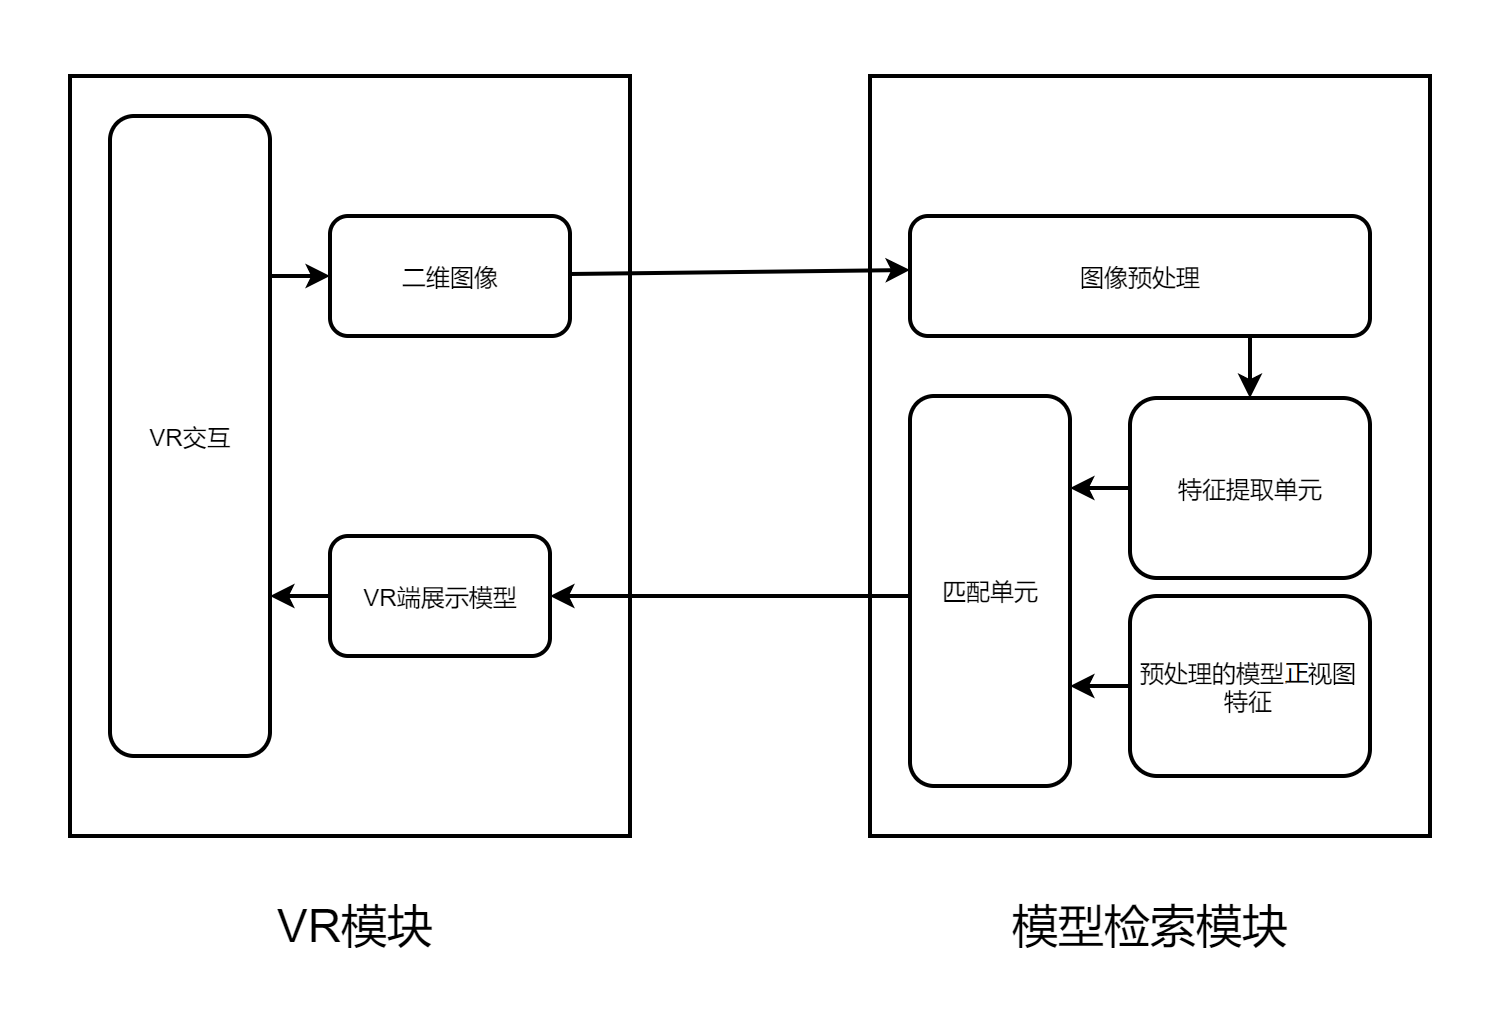
\includegraphics[width=1\textwidth]{images/architecture.png}
\caption{系统架构}\label{fig:digit}
\end{figure} 

\subsection{VR模块}
\subsubsection{设计考虑}
在开题报告中我们首先考虑使用tilt brush在unity中进行开发,用户在VR空间中进行三维的绘图。但在实践阶段遇到了两个问题:
\begin{enumerate}
    \item tilt brush 相关教程较少,他更多是一个开发好了的绘图工具,与unity整合在一起获取画出的模型资源有难度。
    \item 考虑到大部分未经过训练的用户更习惯于普通的在画纸上进行二维创作的习惯,在实践中也会习惯在三维空间里画二维图像.
\end{enumerate}

综合以上考虑,决定对VR端进行这样的设计:在空间中固定一个画板,为用户提供一个可参考的二维平面,然后提供画笔让用户进行绘画。
\subsubsection{设计中的HCI思想}
\begin{enumerate}
    \item 贴近用户习惯
    
    \qquad 从用户的角度出发,考虑方便性:开题时考虑到在三维空间中画三维图更方便,于是设定了 画三维图像→特征提取→转化为二维图像→匹配识别 的流程。但是在实际的实践中,我们发现了一些问题。
    
    \qquad 对于普通的中学生和老师,在未经训练的情况下,更习惯于在二维平面作画,也就是所谓的纸笔作画。三维空间中的凭空绘制虽然也并不难以学习,但是其稳定程度、作画的舒适感相对来说有些不符合人体工程学。
    
    \qquad 我们发现黑板这样一个在三维空间中提供作画平台的工具在中学教室里非常常见,几乎每个人都有机会接触,也有过接触经验。在课程中我们讲到过人的记忆仓库会对一些长期存在的记忆有偏好,一些长期记忆会渐渐规则化、潜意识化。我们人机界面的设计原则中很重要的一点就是要减少学习适应的信息总量,使用用户更为熟悉的固有记忆。我们发现黑板作画放在我们的VR环境中会非常容易接受。

    \item 操作的简洁性
    
    \qquad 去掉碰撞体按钮和UI按钮,让用户直接用手柄事件触发各项功能,不需要瞄准和位移,操作更加简洁。增加射线来进行必要的canvas互动,也符合人的一般习惯。

    \item 操作的便捷性
    
    \qquad 我们根据亲身试验的体验感受,选用了最便捷的左右手的trigger、grip键进行主要功能的操作,在满足按键的便捷性的同时确保各事件的互不冲突。
    
    \item 人性化的反馈
    
    \qquad 尽量保持场景的简单、物体的单一,让用户能自行控制黑板和canvas的隐藏和出现。
    
    \qquad 对于检索反馈,给出多个选项来确保最终可以选到想要的模型。对于预选物体进行高亮和全角度展示,方便用户做出快速的判断和选择
    
\end{enumerate}

\subsection{模型检索模块}
模型检索模块分为如下几个部分:
\begin{itemize}
    \item 图像预处理模块
    \item 特征提取模块
    \item 预处理的模型正视图特征模块
    \item 匹配单元模块
\end{itemize}


\begin{enumerate}
    \item 图像预处理模块

\qquad 图像预处理主要是将VR端输入的信息进行二次处理。

\qquad 在实际的操作过程中我们发现,由于对设备使用不熟练或者误操作,在VR中作画时很容易会将多余的干扰信息引入图片中,例如不小心点上的点、断断续续的线、歪歪扭扭的直线、不闭合的曲线等。
为了降低此类因素给特征提取单元的带来的误差,我们在VR输入和特征提取单元之间加入了图片预处理模块,通过一些图形学操作(腐蚀、膨胀等),提取尽可能清晰、完整的图像轮廓。
    
    
    \item 特征提取模块
    
\qquad 特征提取模块主要目的是提取出VR输入信息中的特征。

\qquad 此模块可以复用从模型三视图中提取特征模块的工程代码。主要目的是找出VR端输入信息中的特征,并以此为基础来匹配出和输入特征重合度较高的模型。
    
    \item 预处理的模型正视图特征模块

\qquad 预处理模型正视图部分存储了已有模型正视图对应的特征值。通过直接使用预处理的模型三视图特征,能够大大降低模型检索耗费的时间。

\qquad 在之前的设计中考虑同时使用正视图/俯视图/侧视图的特征,但是在实验中我们发现,用户在使用简笔画来绘制某种模型时,通常只会绘制正视图,因为正视图包含了最多的形状特征,而且最具独特性。俯视图和侧视图包含的形状特征较少,在不同模型之间还会有重复性。

\qquad 综上所述,我们决定只使用正视图的特征。
    
    \item 匹配模块

\qquad 匹配单元主要通过VR信息提取出的特征值与预处理的模型三视图的特征值来匹配出合适的模型,并返回给VR端。

\end{enumerate}

\section{技术细节}

\subsection{VR模块}

\subsubsection{场景设计}
定义了一个黑板(在场景中建一个Quad)和一支画笔。

\begin{figure}[htb]
    \centering
    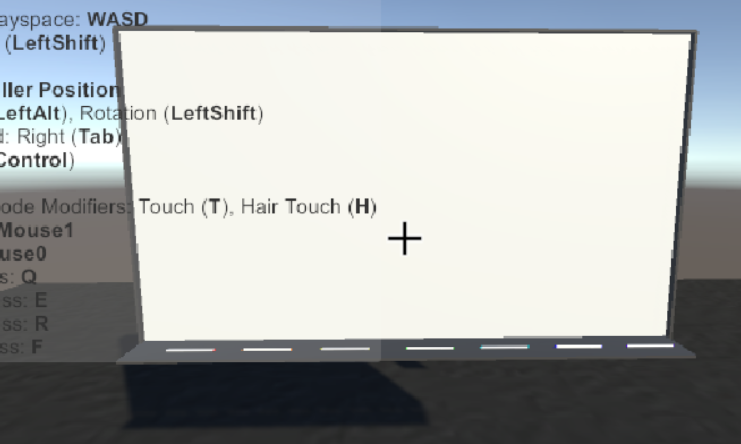
\includegraphics[width=0.8\textwidth]{images/board.png}
    \caption{画板}\label{fig:digit}
\end{figure} 
    
画笔的设计上有些复杂,分为笔的头、尾(控制握笔的方向)还有笔尖(用来绘画)。在画笔触碰到黑板时触发函数记录画笔此刻的位置并将此处的像素点设置颜色,然后实时更新黑板面的texture来显示绘画图案。
    
\begin{figure}[htb]
    \centering
    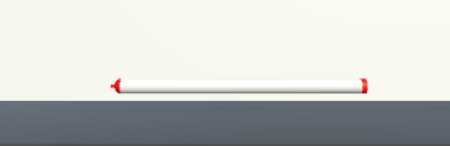
\includegraphics[width=0.8\textwidth]{images/pen.png}
    \caption{画笔}\label{fig:digit}
\end{figure}
    
\subsubsection{功能实现}
\begin{enumerate}
   
    \item 关于像素点绘制: 
    
    运用Unity Texture2D类中的两个函数:
    
\begin{lstlisting}[title=SetPixel, frame=shadowbox]
public void SetPixels32(int x, int y, int blockWidth, int blockHeight, Color32[] colors, int miplevel = 0);
\end{lstlisting}
    
    \qquad 前面4个参数相当于一个矩形,x和y就是矩形的左下角的那个点,blockWidth和blockHeight分别是矩形的宽和高,这个矩形所代表的范围就是blockWidth*blockHeight个像素所在的位置,不妨称这个矩形范围为一个色块;
    
    \qquad colors这个参数的大小必须等于blockWidth*blockHeight,因为这个方法就是给坐标(x,y)开始,从左到右,从下到上,一行一行的对矩形范围内的每个像素赋值;也就是把colors[0]~colors[blockWidth - 1]分别赋值到坐标为(x,y)~(x + blockWidth,y)的像素,以此类推;
    
    \begin{lstlisting}[title=Apply, frame=shadowbox]
public void Apply(bool updateMipmaps = true, bool makeNoLongerReadable = false);
\end{lstlisting}
     
     \qquad 当对图片改动完成以后,需要调用这个方法,才能让改动真正的应用在图片上;
    
    \begin{figure}[htb]
        \centering
        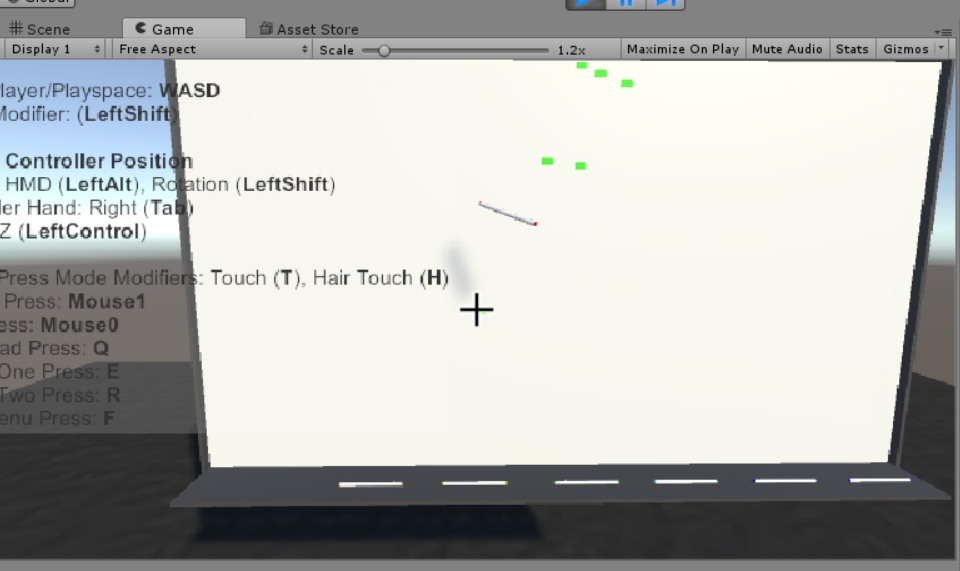
\includegraphics[width=0.7\textwidth]{images/draw.jpg}
        \caption{执笔绘画场景}\label{fig:digit}
    \end{figure} 
    
     
    \item 关于绘画信息传输:
    
    \qquad 当触碰到信息传输的碰撞体时,会将此刻的黑板画面由Texture2D格式转成PNG格式保存下来,用以比对检测。
    
    
    \item 关于模型的展示:
    
    \qquad 当触碰到展示模型的碰撞体时,会在场景中显示prefab库中对应名称(名称信息由检索系统返回)的模型,展示在场景中。
    
\end{enumerate}

\subsubsection{体验优化}
\begin{enumerate}
    \item 防止画笔穿过画板
    
    \qquad 为了让黑板能够绘制图像,board的collider不能设置为box而是设置为mesh,因此会造成笔能穿过黑板的问题。这样会给绘画带来许多不方便之处,不符合人机交互的思想。为了让我们的交互更加符合真实场景,我们给绘画加入一个防止画笔穿过黑板的功能。
    
    \qquad 设计的基本思路是通过检测笔在画板哪一侧来限制笔的位置:
    \begin{itemize}
        \item 给黑板增加一个Plane类型的字段,计算笔尖的点处于Plane的哪一侧,以及到Plane的距离。这样就可以潘断出笔尖是不是穿透了画板,并且可以获取笔尖穿透的距离,从笔尖的位置减去这个距离,则刚好可以让笔尖处于平面上;
        \item 由于目前没有合适的抓附机制来处理穿透的情况,因此需要自己扩展一种抓附机制;直接或者间接继承自VRTK\_BaseGrabAttach,定义了一个VRTK\_InteractableObject的VRTK\_BaseGrabAttach类型的抓起方式字段;
    \end{itemize}

    \item 检索后的信息反馈
    
    \qquad 轮播框的正中间显示检索匹配度最高的模型图片,其余模型图片按匹配度降序向两边分布,可见图片为5个。
    
    \qquad 为了更加美观且体验友好的显示,我们将正中间的图片高亮显示,在上方渲染出该图片对应模型的360°旋转的动态效果。点击正中间的图片即可隐藏canvas,加载模型。

    \qquad 如果所选的图片不在正中间,我们需要点击其他图片,这时轮播框将会转动,将我们选定的图片移到正中间进行高亮显示。
    
    \begin{figure}[htb]
        \centering
        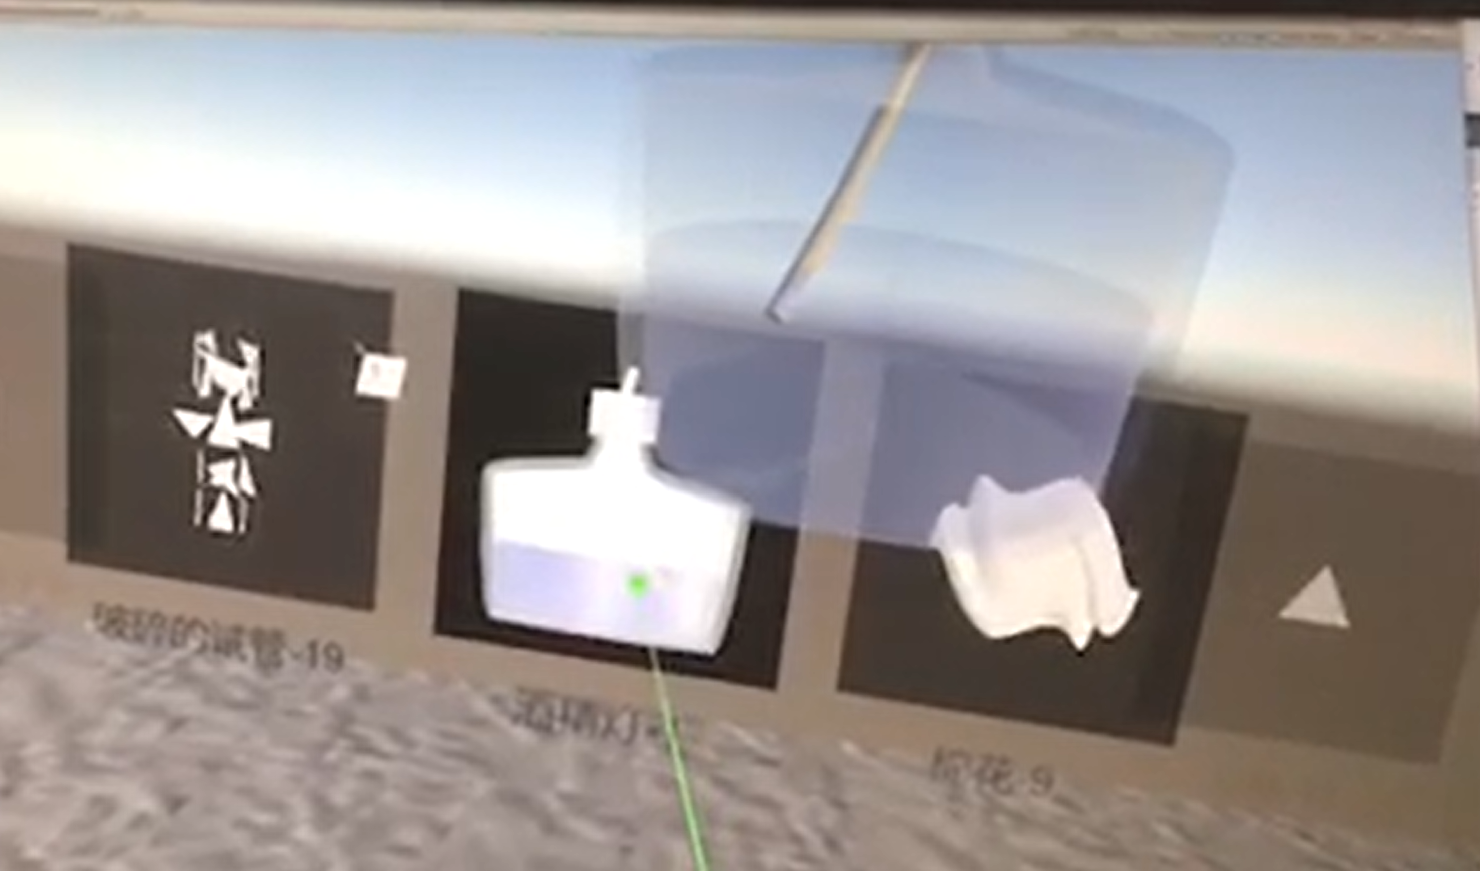
\includegraphics[width=0.7\textwidth]{images/VR.png}
        \caption{VR场景中的轮播展示}\label{fig:digit}
    \end{figure} 
    
    \item 更加友好的手柄交互体验
    
    \qquad 在VR中我们主要通过手柄来进行各项操作。对于手柄交互的便捷性我们做出了如下改进:
     \begin{itemize}
        \item 画完图像之后点击左手柄的trigger键便触发检索流程,此时黑板被隐藏,canvas被调出并显示检索结果。
        \item 使用右手柄的trigger键调出射线,用右手柄的grip键选中图片。
        \item 用左手柄的grip键来重新调出黑板进行下一轮作画,此时的黑板已经被清空。
        \item 在绘画过程中可以按压左手柄的touchpad来将不满意的绘画清空。
        \item 给画笔触碰到黑板的第一下加入了声响。这在一部分曾经尝试使用手柄震动,但震动会对绘画有一定的影响。此外长时间的接触声响也会影响用户体验,因此我们在每一笔第一次触碰黑板时才发出碰撞声响,提示用户画笔已经就位。
    \end{itemize}
    
\end{enumerate}
\subsection{模型检索模块}
模型检索部分完成了以下工作:
\begin{itemize}
    \item 模型正视图渲染
    \item 对模型正视图/VR简笔画进行预处理
    \item 傅里叶轮廓描述符提取
    \item 特征匹配
\end{itemize}

\subsubsection{模型正视图渲染}
使用可编程的Blender软件设置渲染场景,并使用Python脚本进行模型加载、渲染参数设置,最终渲染得到模型的正视图

\begin{figure}[htb]
    \centering
    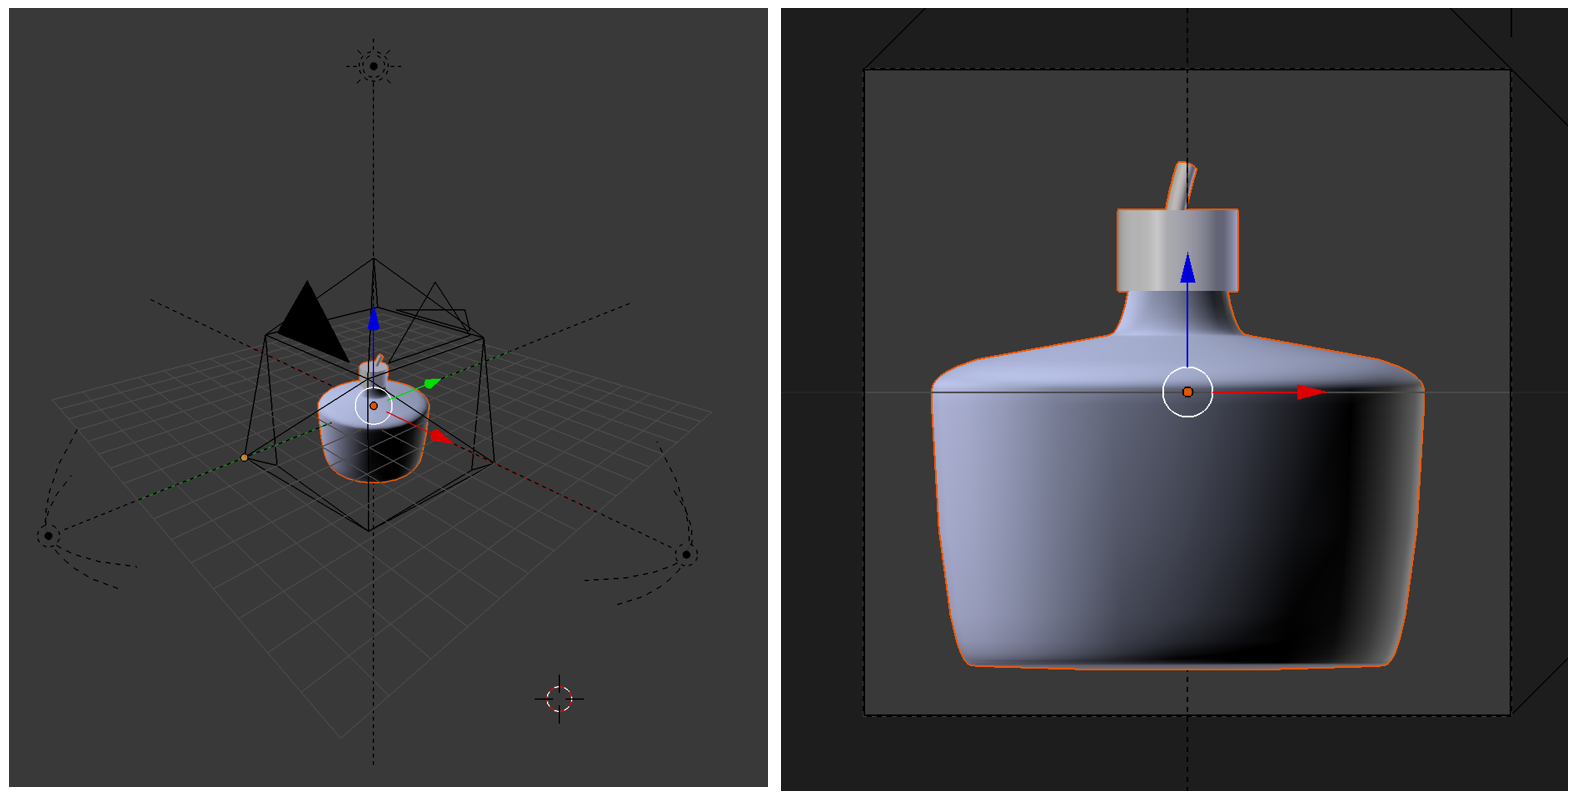
\includegraphics[width=0.8\textwidth]{images/Blender.png}
    \caption{模型正视图渲染}\label{fig:digit}
\end{figure} 
    
由于模型的部分材质是玻璃或者水这样的透明物质,所以我们对模型进行了一些调整,改变了部分Material的高光、透明度、颜色等参数。同时为了渲染出位置、大小合适的图像,对模型的重心和尺寸也进行了调整。

\subsubsection{图像预处理}
为了去除原始图像中的噪声,并提取得到清晰完整的轮廓,对图像进行了以下处理

\begin{enumerate}
    \item 将RGB/RGBA图像转化成灰度图像,去除颜色信息的干扰
    \item 使用Canny算子检测图像中的轮廓,得到包含内外轮廓的二值图像
    \item 对轮廓进行膨胀操作,使断断续续的边缘连接成一个整体
    \item 提取图像中轮廓点集
    \item 根据包含的点数对轮廓列表进行排序,保留点最多的一个轮廓,这样做的目的是排除误操作产生的散点的干扰
\end{enumerate}

\begin{figure}[htb]
    \centering
    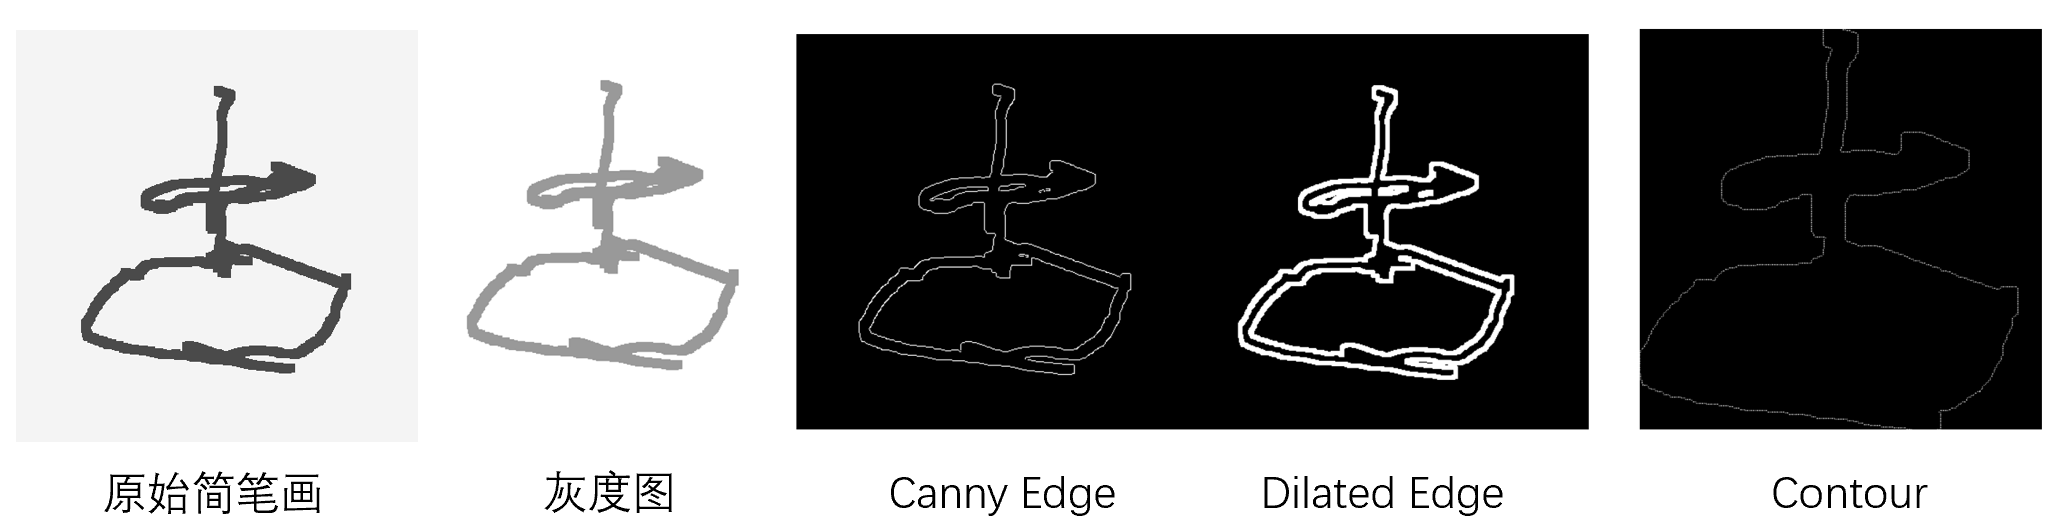
\includegraphics[width=0.8\textwidth]{images/contour.png}
    \caption{图像预处理各阶段效果}\label{fig:digit}
\end{figure} 

\subsubsection{傅里叶轮廓描述符提取}
傅里叶描述符(Fourier Descriptor)将物体的形状看做是一条封闭的曲线,称为边界曲线。把曲线上的点(x,y)表示为复数形式(x+yi),就可以把边界曲线看作描述点变化的周期函数,这个函数用傅里叶级数展开,将得到一系列复数形式的系数,它们共同描述了边界的形状。

\begin{figure}[htb]
    \centering
    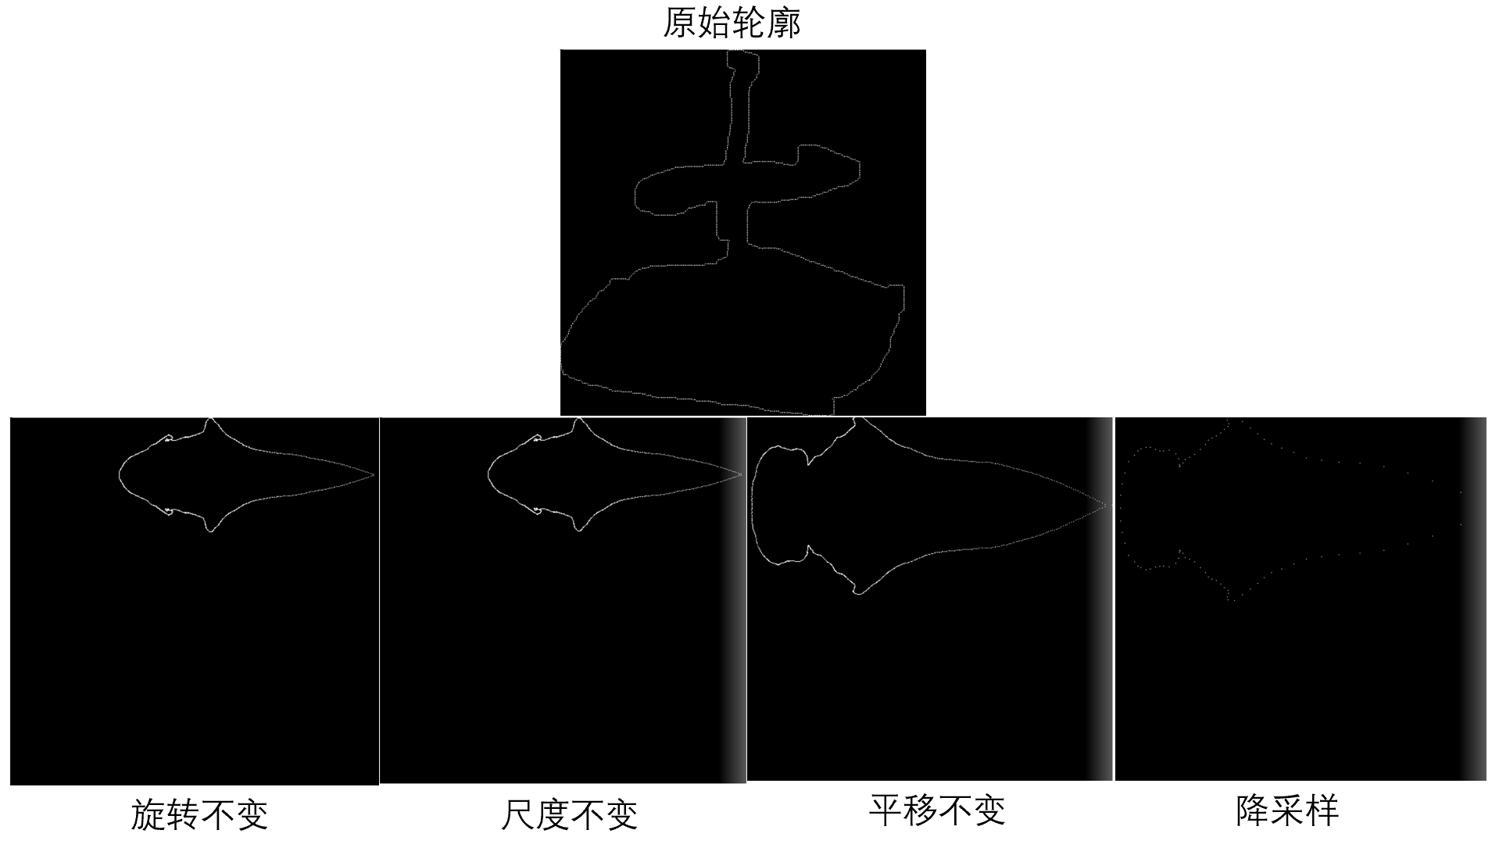
\includegraphics[width=0.8\textwidth]{images/Fourier.png}
    \caption{傅里叶轮廓描述符}\label{fig:digit}
\end{figure} 

之前的实现中只是提取了原始的描述符并进行了降采样操作,现在还加入了旋转不变、尺度不变、平移不变的处理,使描述符更robust,极大的提高了匹配的准确率。

\subsubsection{特征匹配}   
之前的实现中尝试了使用SVM和KNN进行匹配,但是这两种方法需要大量的训练数据,考虑到我们资源的有限性,就舍弃了这两种方法。

由于特征描述符的可靠性获得了极大的提高,现在采用了计算L1距离,根据距离进行升序排序的方法。这样的方法极大减少了计算量,还保持了令人满意的匹配准确率,使模型检索兼具时效性和准确性。

\subsection{模块整合}
将Unity和python后端进行整合,需要完成以下工作:

\begin{enumerate}
    \item 使用C\#脚本调用python脚本,并对返回结果进行解析
    \item 将模型检索的结果进行展示
\end{enumerate}

\subsubsection{Unity中调用python}
使用了System.Diagnostics命名空间下的Process控件调用python脚本。具体流程如下:
\begin{enumerate}
    \item VR中绘制了简笔画之后,把简笔画存到本地
    \item 把python脚本的路径和简笔画图片的路径当作参数,调用python执行文件
    \item 在python脚本中把匹配结果编码为字符串,print出来,Unity中把这一输出进行重定向,就可以获得输出字符串
    \item 对字符串进行解析,就可以的到模型检索结果
\end{enumerate}

\subsubsection{模型检索结果可视化}
在得到模型匹配的结果后,需要用一种美观且用户友好的方式进行展示

我们对具体的展示方法进行了两次尝试:
\begin{enumerate}
    \item 第一次尝试
    
    \qquad 只展示排序靠前的5个模型的图片,用户可以点击自己想要的结果来获得模型
    
    \begin{figure}[htb]
        \centering
        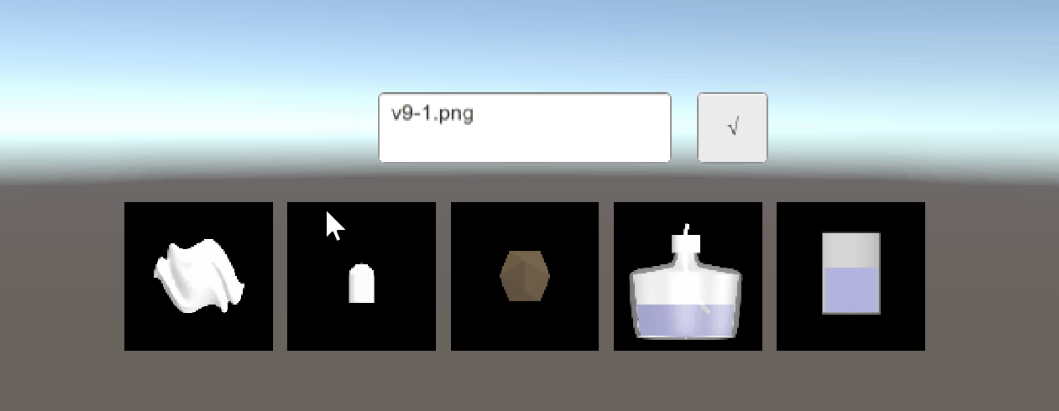
\includegraphics[width=0.8\textwidth]{images/version1.png}
        \caption{初步可视化效果}\label{fig:digit}
    \end{figure} 
    
    \qquad 这样的可视化方法有以下缺陷:
    \begin{enumerate}
        \item 只能显示5个候选模型,如果目标模型不在其中,就必须重新绘制简笔画
        \item 只显示了模型正视图,有的时候难以确定到底是什么模型
    \end{enumerate}
    
    \item 第二次尝试
    
    \qquad 使用一个轮播框(Scroll Flow)来展示检索结果,最开始的时候按照排序结果把最接近的模型排在最前方,如果目标模型不在几个候选中,用户可以选择左右切换其他模型,也可以选择重新绘制简笔画
    
    \qquad 另外设置了一个相机围绕模型进行旋转,将相机拍摄到的画面作为纹理贴在一个Raw Image上,这样就可以在切换模型图片的同时看到全角度的模型画面,方便用户进行选择
    
    \qquad 把模型的名称显示在图片的下方,提供了额外的信息方便用户进行选择
    
    \begin{figure}[htb]
        \centering
        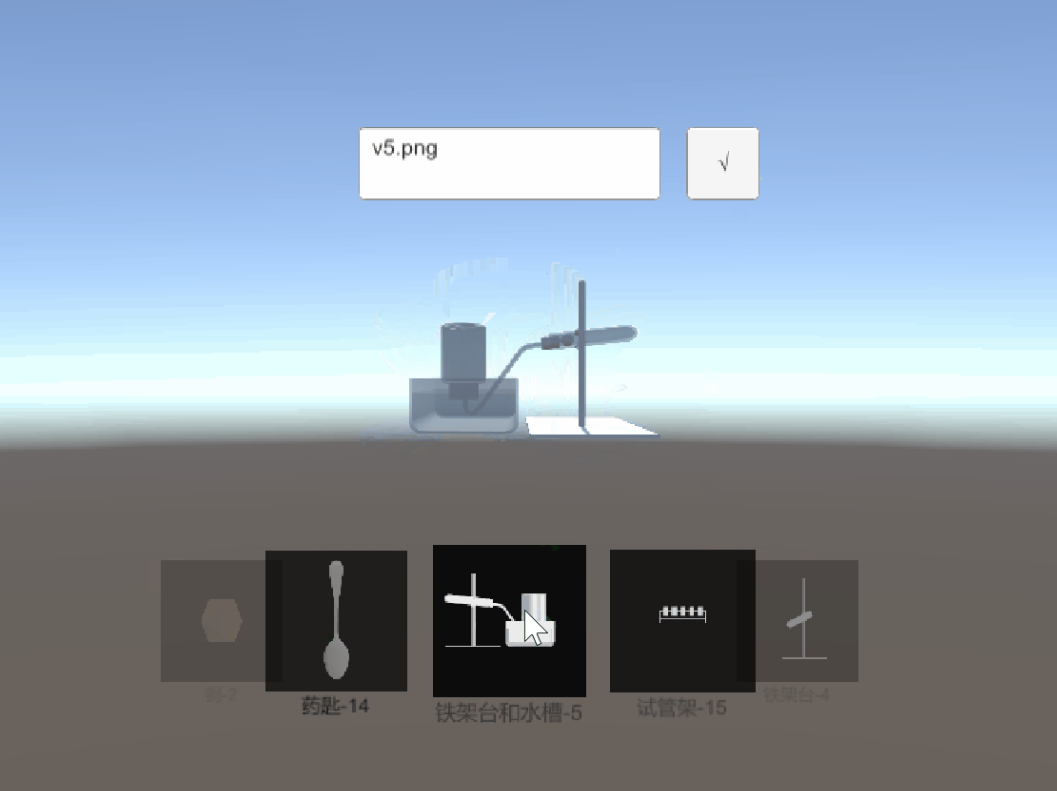
\includegraphics[width=0.8\textwidth]{images/version2.png}
        \caption{改进后可视化效果}\label{fig:digit}
    \end{figure} 
    
\end{enumerate}

\section{实验验证}
对模型检索的准确性和时效性进行了实验验证
\begin{enumerate}
    \item 数据:使用已有的20个模型的正视图轮廓特征作为匹配数据库,对VR端绘制得到的15张简笔画进行特征匹配
    \item 变量:不同描述符度数
    \item 测试指标:(1)匹配用时(2)正确结果在输出的排序结果中的位置
\end{enumerate}
\subsection{实验数据}

\begin{figure}[htb]
    \centering
    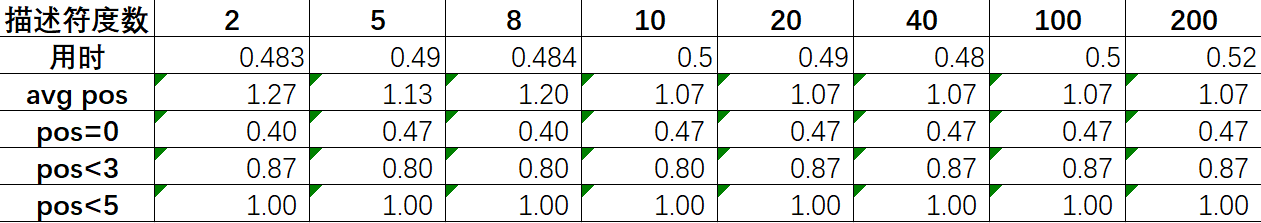
\includegraphics[width=0.8\textwidth]{images/data.png}
    \caption{实验数据}\label{fig:digit}
\end{figure} 

\begin{enumerate}
    \item 用时:匹配15个模型的总耗时 \\
    \item avg pos:平均检索结果中正确模型的位置 \\
    \item 后三行:模型出现在第一位/前三位/前五位的概率 \\
\end{enumerate}

\subsection{结果分析}

\subsubsection{检索时效性}

\begin{figure}[htb]
    \centering
    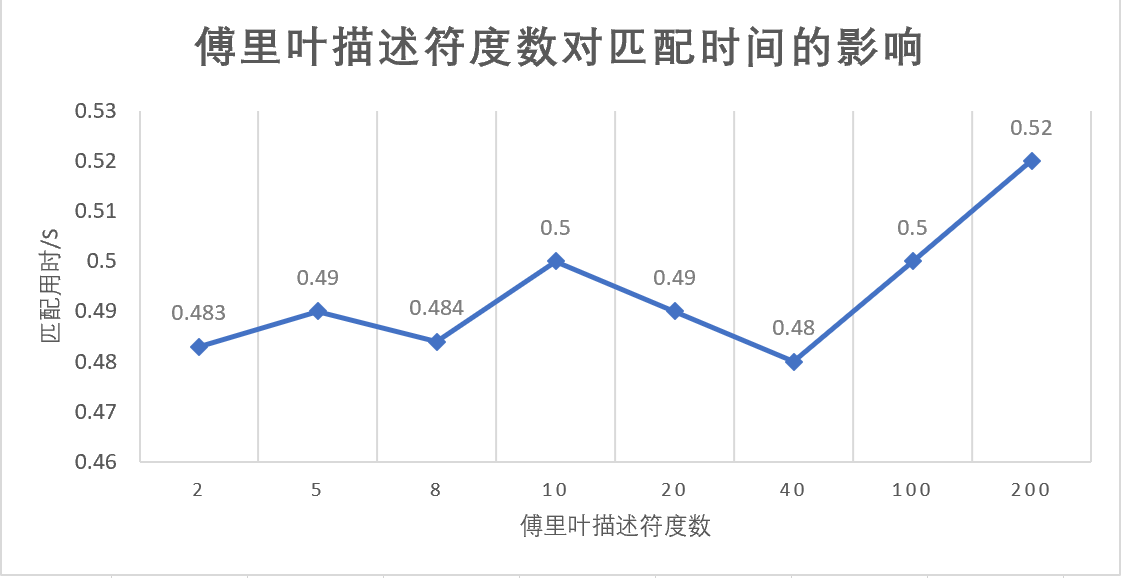
\includegraphics[width=0.8\textwidth]{images/time.png}
    \caption{检索时效性}\label{fig:digit}
\end{figure} 

\begin{enumerate}
    \item 可见时间都在0.5s左右,而且这是匹配15个模型的总用时,单个模型的话会略短一些
    \item 可以认为满足时效性的要求,在实际运行时模型检索耗时不会影响用户的体验
\end{enumerate}

\subsubsection{检索可靠性}

\begin{enumerate}
    \item 15个简笔画检索出的正确模型出现在前五个的几率是百分之百,可以在轮播框的直接显示结果中选中目标模型
    \item 描述符度数>10之后,检索的精度就不再提升,因此将来如果需要进一步优化性能,可以考虑适当降低描述符度数
    \item 可以认为满足准确性的要求,实际运行时基本不需要切换轮播框页,就可以得到正确的模型
\end{enumerate}

\begin{figure}[htb]
    \centering
    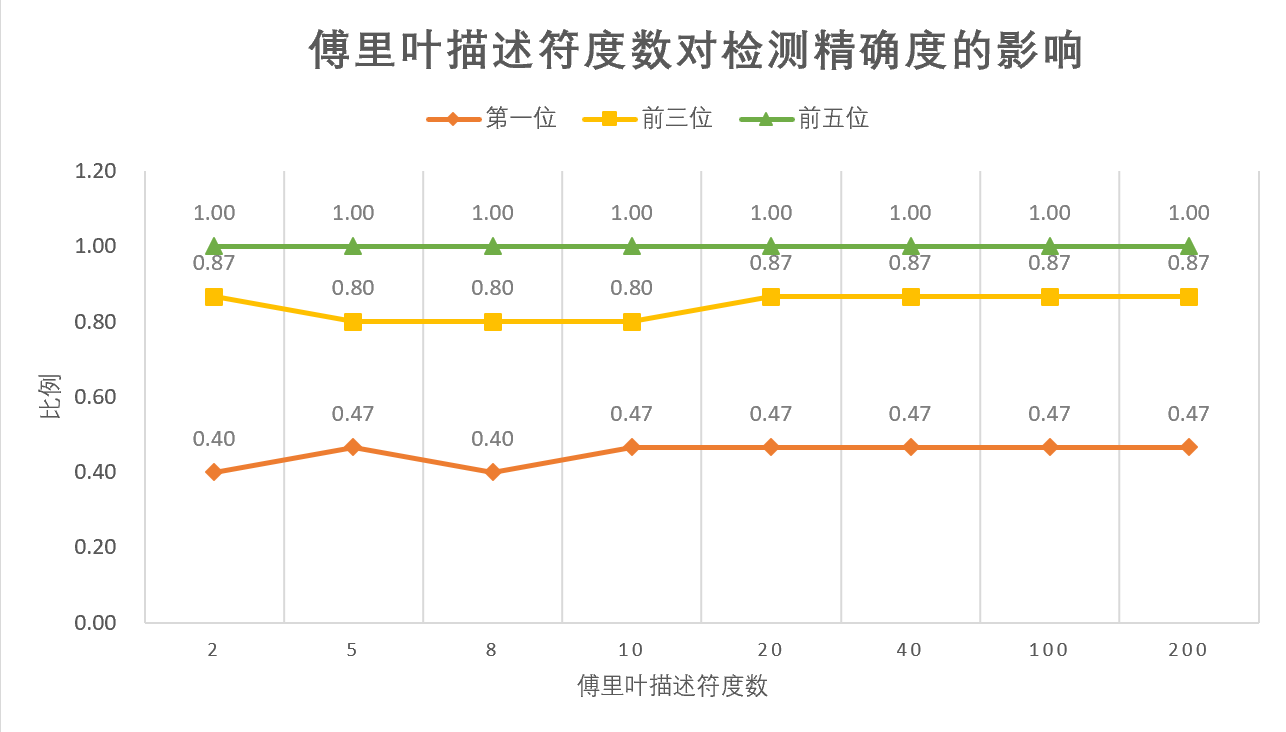
\includegraphics[width=0.8\textwidth]{images/precision.png}
    \caption{检索可靠性}\label{fig:digit}
\end{figure} 


\section{环境配置}
模型检索模块:
\begin{itemize}
    \item 环境:python2.7
    \item 依赖:OpenCV-dev,Numpy
\end{itemize}

VR模块:
\begin{itemize}
    \item VRTK
\end{itemize}

Unity版本: \\
2018.3.1f1 (64-bit)

\section{项目分工及推进}
\subsection{项目分工}
\subsubsection{12-14周}

\begin{center}
    

\begin{tabular}{ccc}
\hline
姓名& 学号& 工作\\
\hline
陈志扬& 516030910347& VR端优化\\
罗宇辰& 516030910101& 特征匹配\\
陈诺 & 516030910199 & VR端简笔画预处理 \\
\hline
\end{tabular}

\subsubsection{13-16周}
\begin{tabular}{ccc}
\hline
姓名& 学号& 工作\\
\hline
陈志扬& 516030910347& VR端与模型检索端连接\quad 实验室调试 \quad 答辩PPT\\
罗宇辰& 516030910101& 特征匹配实验 \quad 实验室调试 \quad 终期报告\\
陈诺 & 516030910199 & 实际环境下VR交互优化 \quad 实验室调试 \quad demo录制剪辑与教程视频 \quad\\
\hline
\end{tabular}

\end{center}

\subsection{项目推进}
\begin{itemize}
    \item 每周二下午小组会议制定本周计划
    \item 每周五晚上小组会议商讨计划进度,及时修改计划
\end{itemize}

\section{致谢}
   
\thispagestyle{empty}
感谢肖老师严谨授课,感谢肖助教的技术指导,感谢dalab成员对于VR设备使用的支持。

\clearpage


\end{document}
